% Options for packages loaded elsewhere
\PassOptionsToPackage{unicode}{hyperref}
\PassOptionsToPackage{hyphens}{url}
%
\documentclass[
]{article}
\usepackage{amsmath,amssymb}
\usepackage{lmodern}
\usepackage{ifxetex,ifluatex}
\ifnum 0\ifxetex 1\fi\ifluatex 1\fi=0 % if pdftex
  \usepackage[T1]{fontenc}
  \usepackage[utf8]{inputenc}
  \usepackage{textcomp} % provide euro and other symbols
\else % if luatex or xetex
  \usepackage{unicode-math}
  \defaultfontfeatures{Scale=MatchLowercase}
  \defaultfontfeatures[\rmfamily]{Ligatures=TeX,Scale=1}
\fi
% Use upquote if available, for straight quotes in verbatim environments
\IfFileExists{upquote.sty}{\usepackage{upquote}}{}
\IfFileExists{microtype.sty}{% use microtype if available
  \usepackage[]{microtype}
  \UseMicrotypeSet[protrusion]{basicmath} % disable protrusion for tt fonts
}{}
\makeatletter
\@ifundefined{KOMAClassName}{% if non-KOMA class
  \IfFileExists{parskip.sty}{%
    \usepackage{parskip}
  }{% else
    \setlength{\parindent}{0pt}
    \setlength{\parskip}{6pt plus 2pt minus 1pt}}
}{% if KOMA class
  \KOMAoptions{parskip=half}}
\makeatother
\usepackage{xcolor}
\IfFileExists{xurl.sty}{\usepackage{xurl}}{} % add URL line breaks if available
\IfFileExists{bookmark.sty}{\usepackage{bookmark}}{\usepackage{hyperref}}
\hypersetup{
  pdftitle={Supplementary figures},
  hidelinks,
  pdfcreator={LaTeX via pandoc}}
\urlstyle{same} % disable monospaced font for URLs
\usepackage[margin=1in]{geometry}
\usepackage{graphicx}
\makeatletter
\def\maxwidth{\ifdim\Gin@nat@width>\linewidth\linewidth\else\Gin@nat@width\fi}
\def\maxheight{\ifdim\Gin@nat@height>\textheight\textheight\else\Gin@nat@height\fi}
\makeatother
% Scale images if necessary, so that they will not overflow the page
% margins by default, and it is still possible to overwrite the defaults
% using explicit options in \includegraphics[width, height, ...]{}
\setkeys{Gin}{width=\maxwidth,height=\maxheight,keepaspectratio}
% Set default figure placement to htbp
\makeatletter
\def\fps@figure{htbp}
\makeatother
\setlength{\emergencystretch}{3em} % prevent overfull lines
\providecommand{\tightlist}{%
  \setlength{\itemsep}{0pt}\setlength{\parskip}{0pt}}
\setcounter{secnumdepth}{-\maxdimen} % remove section numbering
\ifluatex
  \usepackage{selnolig}  % disable illegal ligatures
\fi

\title{Supplementary figures}
\author{}
\date{\vspace{-2.5em}}

\begin{document}
\maketitle

\hypertarget{targeted-and-untargeted-proteomics-of-plasma-from-cord-blood-with-high-vs-low-hematopoietic-stem-and-progenitor-cell-count}{%
\subsection{Targeted and untargeted proteomics of plasma from cord blood
with high vs low hematopoietic stem and progenitor cell
count}\label{targeted-and-untargeted-proteomics-of-plasma-from-cord-blood-with-high-vs-low-hematopoietic-stem-and-progenitor-cell-count}}

\emph{Anders K Nilsson}†1, Halfdan Rydbeck\emph{1, Annika Thorsell2,
Sofia Frändberg3,4, Helena Barreto Henriksson3,4, Camilla Hesse3,4,
Gunnel Hellgren1,5, Anna-Lena Hård af Segerstad Boberg1, Pia Lundgren6,
and Ann Hellström1 In order to center text in md files you can use the
center tag like html tag: }

\begin{enumerate}
\def\labelenumi{\arabic{enumi})}
\tightlist
\item
  Department of Clinical Neuroscience, Institute of Neuroscience and
  Physiology, Sahlgrenska Academy, University of Gothenburg, Gothenburg,
  Sweden;
\item
  Proteomics Core Facility at Sahlgrenska Academy, University of
  Gothenburg, SE- 40530 Gothenburg, Sweden;
\item
  Department of Clinical Immunology and Transfusion Medicine,
  Sahlgrenska Hospital, Gothenburg, Sweden;
\item
  Department of Obstetrics, The Queen Silvia Children´s Hospital,
  Gothenburg, Sweden;
\item
  Institute of Biomedicine, Sahlgrenska Academy, University of
  Gothenburg, Gothenburg, Sweden;
\item
  School of Medical Sciences, Faculty of Medicine and Health, Örebro
  University, Örebro, Sweden.
\end{enumerate}

Address correspondence to Anders K. Nilsson,
\href{mailto:anders.k.nilsson@gu.se}{\nolinkurl{anders.k.nilsson@gu.se}}

\hypertarget{r-setup-includefalse-my_wdusersxrydbhpersonalprojectsgit_clonedneored_cloned-knitropts_knitsetroot.dir-my_wd}{%
\section{\texorpdfstring{\texttt{\{r,\ setup,\ include=FALSE\}\ \#\ my\_wd="/Users/xrydbh/Personal/Projects/git\_cloned/Neored\_cloned"\ \#\ knitr::opts\_knit\$set(root.dir\ =\ my\_wd)\ \#}}{\{r, setup, include=FALSE\} \# my\_wd="/Users/xrydbh/Personal/Projects/git\_cloned/Neored\_cloned" \# knitr::opts\_knit\$set(root.dir = my\_wd) \#}}\label{r-setup-includefalse-my_wdusersxrydbhpersonalprojectsgit_clonedneored_cloned-knitropts_knitsetroot.dir-my_wd}}

\hypertarget{box-plots-ms}{%
\subsection{Box plots MS}\label{box-plots-ms}}

\hypertarget{fig.s1}{%
\subsection{Fig.S1}\label{fig.s1}}

\begin{figure}
\centering
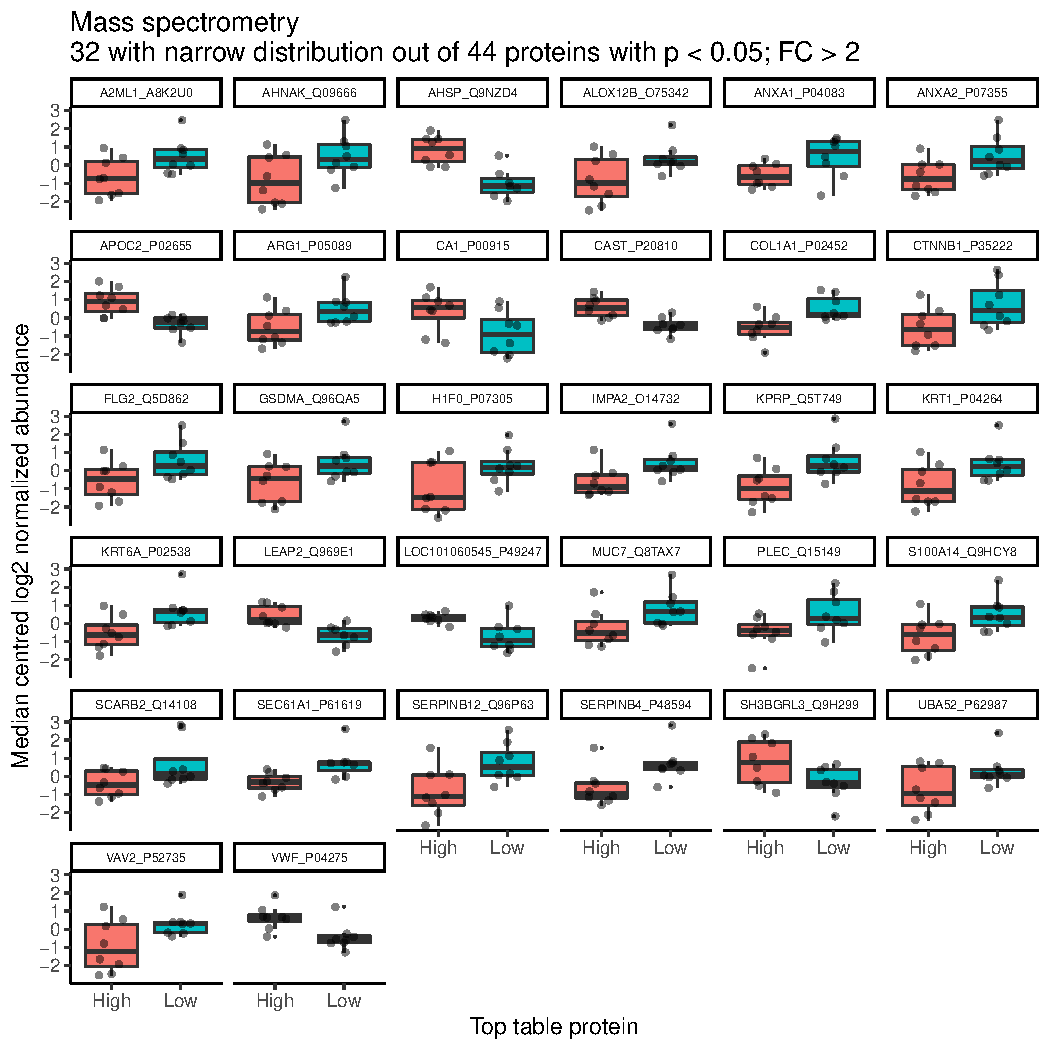
\includegraphics[width=1\textwidth,height=\textheight]{../out_r/008_boxplot_p005_FC_2_sign_DEqMS_narrow_dist_eq_med_norm.pdf}
\caption{Fig.S1 Box plots of proteins in the MS data with
\textgreater two-fold abundance differences and p\textless0.05 between
groups (CD34 high vs CD34 low).}
\end{figure}

\begin{figure}
\centering
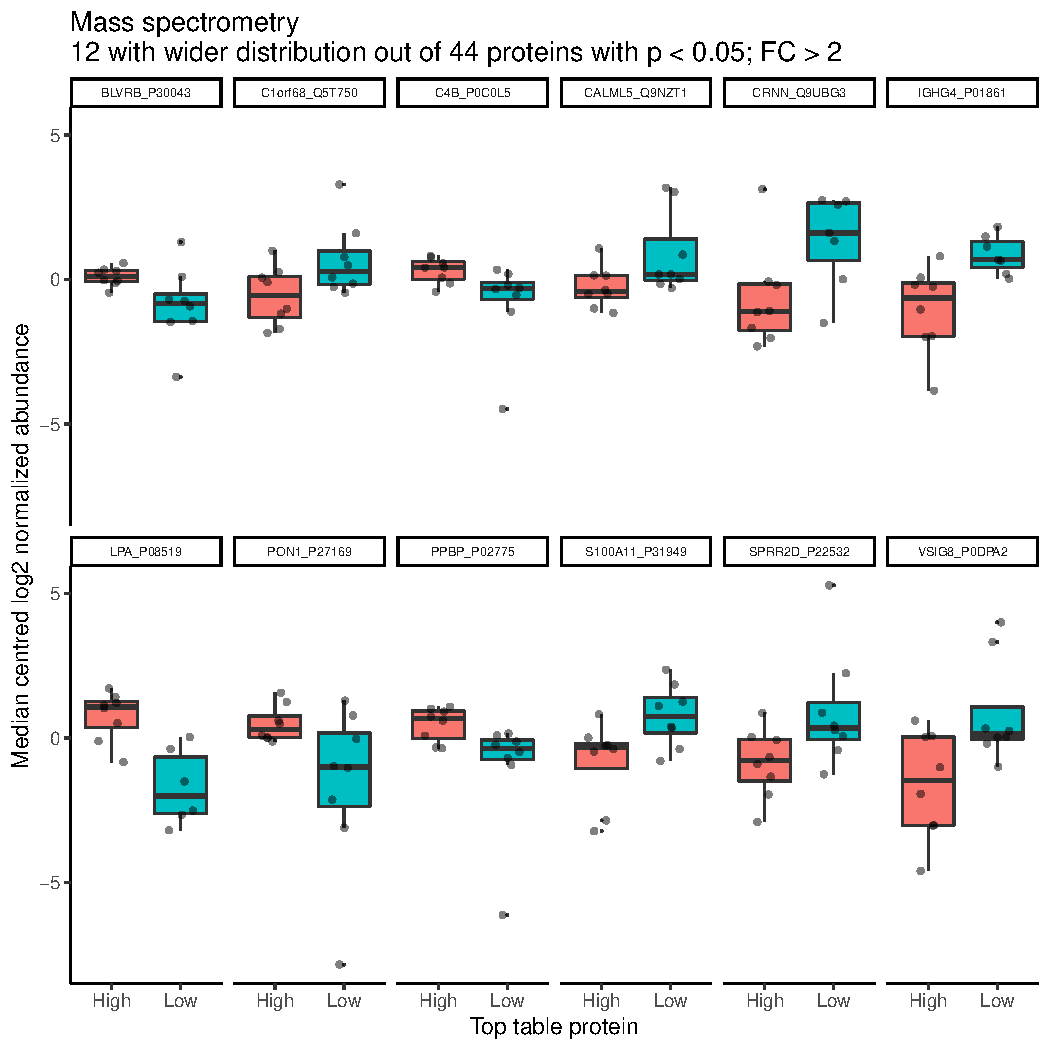
\includegraphics[width=1\textwidth,height=\textheight]{../out_r/008_boxplot_p005_FC_2_sign_DEqMS_wider_dist_eq_med_norm.pdf}
\caption{Fig.S1}
\end{figure}

\hypertarget{fig.s2}{%
\subsection{Fig.S2}\label{fig.s2}}

\begin{figure}
\centering
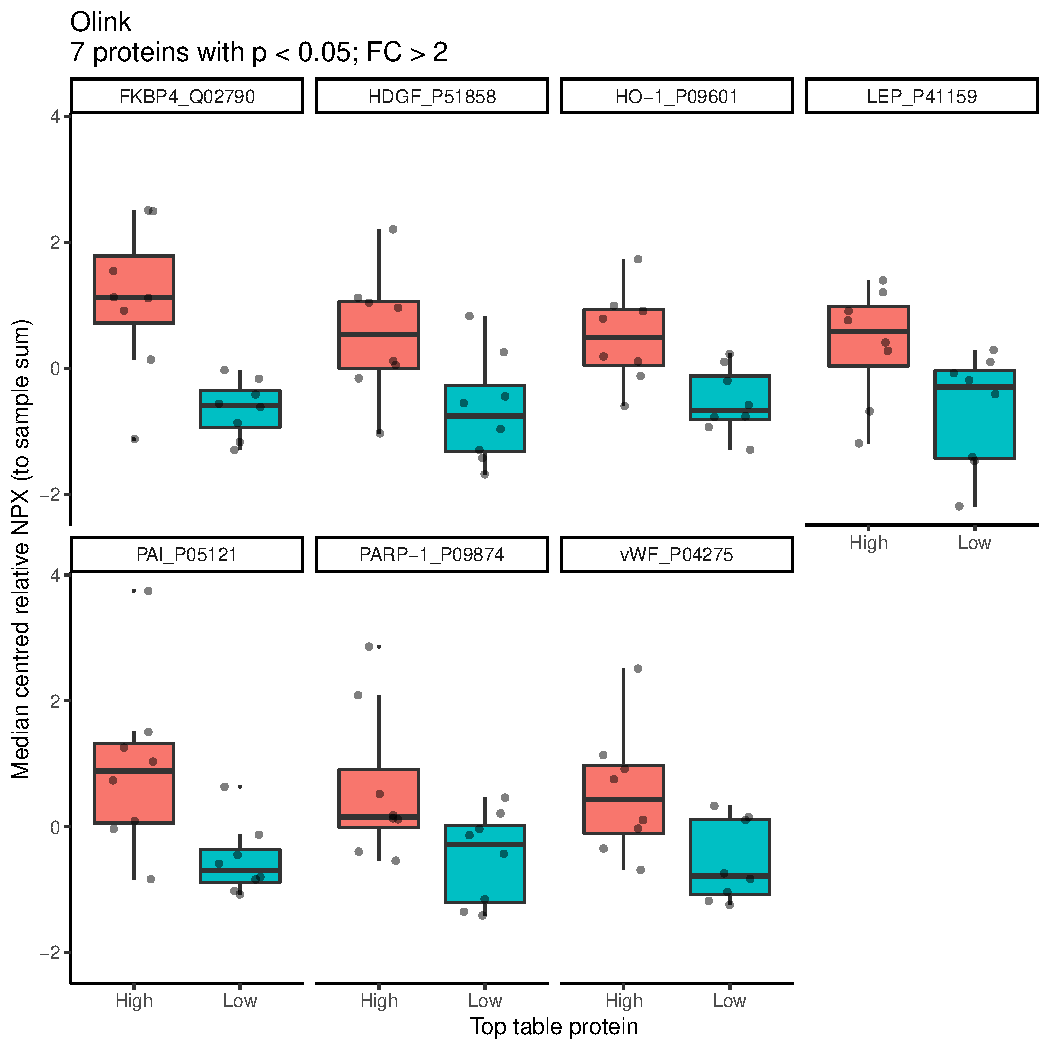
\includegraphics[width=1\textwidth,height=\textheight]{../out_r/008_boxplot_p005_FC_2_sign_ttest_pea_eq_med_norm.pdf}
\caption{Fig.S2}
\end{figure}

\hypertarget{significant_pathways_in_pw_hierarchy}{%
\subsection{Significant\_pathways\_in\_pw\_hierarchy}\label{significant_pathways_in_pw_hierarchy}}

\begin{figure}
\centering
\includegraphics{../out_r/Reactome/Significant_pathways_in_pw_hierarchy.pdf}
\caption{Fig.S3}
\end{figure}

\hypertarget{venn-diagram-of-pathway-overlap}{%
\subsection{Venn diagram of pathway
overlap}\label{venn-diagram-of-pathway-overlap}}

\begin{figure}
\centering
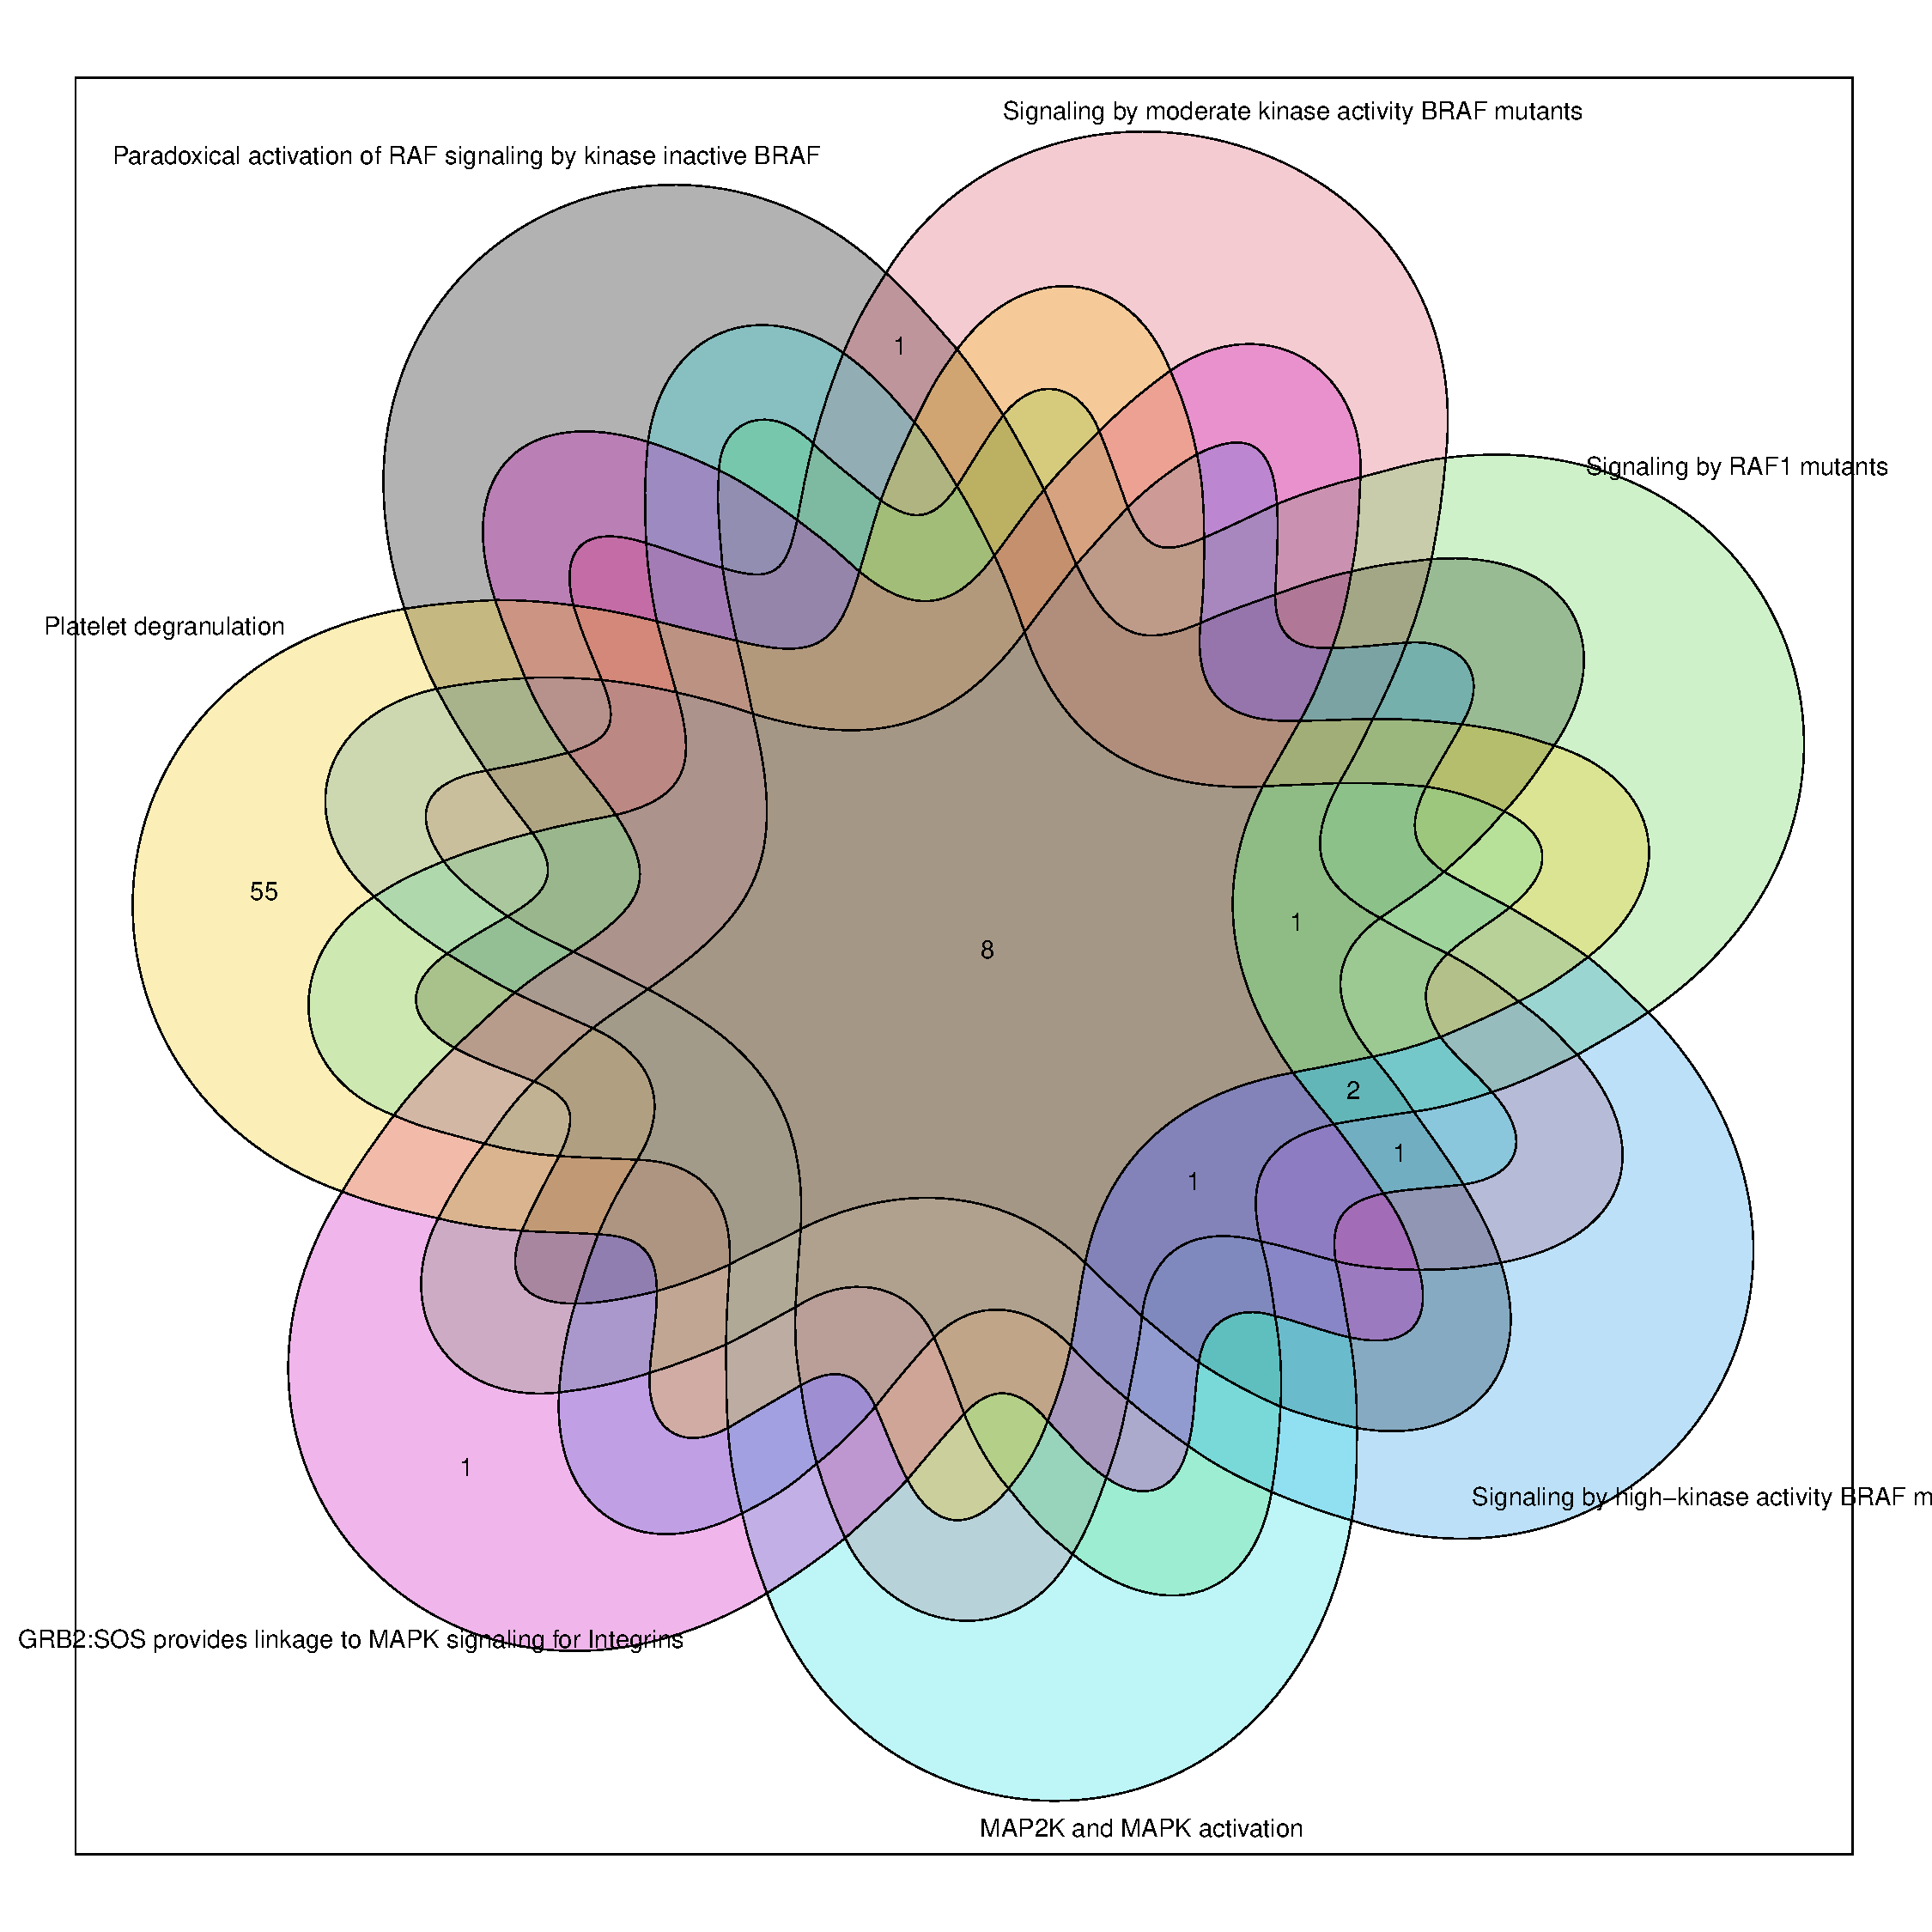
\includegraphics{../out_r/14_venn_pw_overlap_3.pdf}
\caption{Fig.S4}
\end{figure}

\end{document}
